\documentclass[12pt,compress,ngerman,utf8,t]{beamer}
\usepackage{etex}
\usepackage[ngerman]{babel}
\usepackage{graphicx}
\usepackage[export]{adjustbox}
\usepackage{multicol}


\usetheme[numbering=fraction, progressbar=frametitle]{metropolis}


\date{\today}
\institute{University of Freiburg}
\titlegraphic{\hspace{9cm} 
\includegraphics[height=2cm]{template/Logo-Uni-Freiburg.png}}
\graphicspath{ {./template/} {./strategy/} }

\title{Strategie}
\author{Felix Karg}
\subject{Mathecamp}

\newif\ifonline
\onlinefalse
% \onlinefalse

\AtBeginSection[]
{
    \begin{frame}{Inhalt}
        \begin{multicols}{2}
            \tableofcontents[currentsection]
        \end{multicols}
        \clearpage
    \end{frame}
}

\AtBeginSubsection[]
{
    \begin{frame}{Inhalt}
        \begin{multicols}{2}
            \tableofcontents[currentsection,currentsubsection]
        \end{multicols}
        \clearpage
    \end{frame}
}

% \vspace{0.1cm}

\begin{document}


\begin{frame}[c]{Inferentielle Entfernungen}
    % Gedankenschritte
    \large
    Was sind Inferentielle Entfernungen? \\ \pause
    Wir erwarten dass diese kurz sind. Sind sie (meist) nicht.
\end{frame}


\begin{frame}[standout]
    Ganz viele Fragen stellen!
\end{frame}


\maketitle

% multicols from:
% https://tex.stackexchange.com/questions/24343/splitting-toc-into-two-columns-on-single-frame-in-beamer

%%%%%%%%%%%%%%%%%%%%%%%%%%%%%%%%%%%%%%%%%%%%%%%%%%%%%%%%%%%%%%%%%%%%%%%%%%%%%%%%%%%%%%%%%%%%%%%%%%%%%%%%%%%%%%%%%%%

\begin{frame}{Inhalt}
    \small
    \begin{multicols}{2}
        \small
        \tableofcontents[hidesubsections]
    \end{multicols}
    \clearpage
\end{frame}




%%%%%%%%%%%%%%%%%%%%%%%%%%%%%%%%%%%%%%%%%%%%%%%%%%BEGINNING%%%%%%%%%%%%%%%%%%%%%%%%%%%%%%%%%%%%%%%%%%%%%%%%%%%%%%%%
\section{Recap}



\begin{frame}[c]{}
    \center
    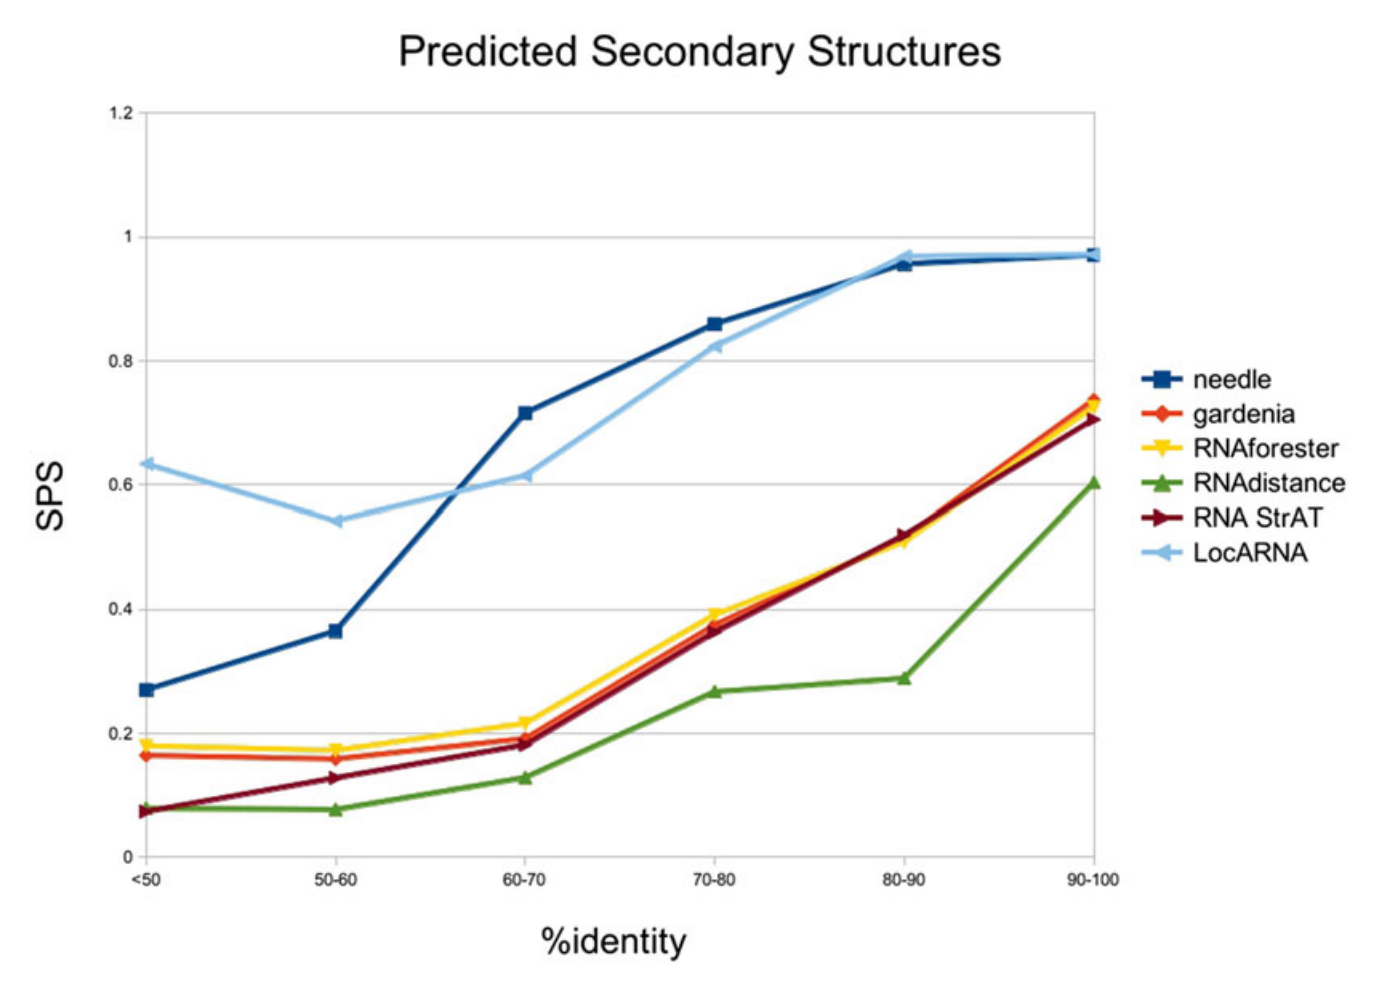
\includegraphics[width=\textwidth]{predicted}
\end{frame}


\begin{frame}[c]{}
    \center
    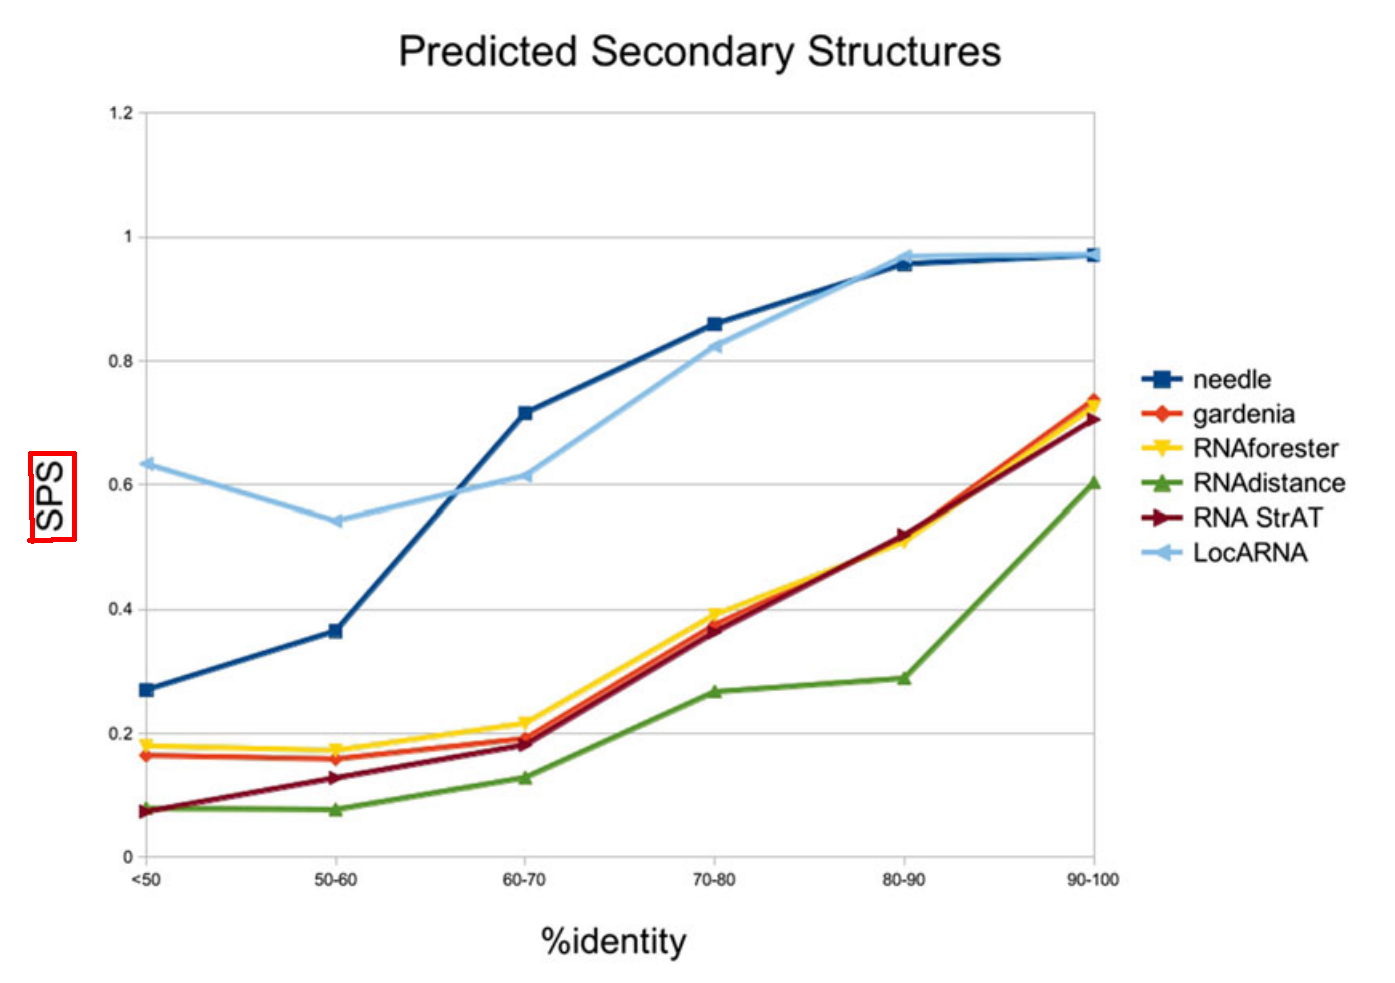
\includegraphics[width=\textwidth]{predicted_sps}
\end{frame}


\begin{frame}[c]{SPS - introduction}
    Sum of Pairs Score
    \newline
%    \vspace{2cm}
    \newline
    \pause
    Used to measure the \only<2-2>{alignment}\only<3->{similiarity} of two RNA sequences
\end{frame}


\begin{frame}[c]{Sequence Similiarity - Example}
    A: \only<4-5>{AAGGC}\only<1-1>{AAGGC}\only<2-3>{{\color{ForestGreen} AAGGC}}\only<1,4->{TT}\only<2-3>{{\color{red}TT}} \\
    B: \only<1-1>{AAGGC}\only<2-5>{{\color{ForestGreen} AAGGC}} \\
    C: \only<1-3>{AAGGC}\only<4->{{\color{ForestGreen} AAGGC}}\only<4-5>{{\color{red}AT}}\only<-3>{AT} \newline
    \newline
    Similiarity: \only<3,5>{60\% = 1 - (2 / 5) } \\
    1 - (edit distance / unaligned length of shorter sequence)
\end{frame}


\begin{frame}[c]{Sequence Similiarity - Example}
    A: {\color{ForestGreen}AAGGC}{\color{red}T}{\color{ForestGreen}T} \\
    B: AAGGC \\
    C: {\color{ForestGreen}AAGGC}{\color{red}A}{\color{ForestGreen}T} \newline
    \newline
    Similiarity: \only<2>{ 86\% = 1 - (1 / 7) } \\
    1 - (edit distance / unaligned length of shorter sequence)
\end{frame}


\begin{frame}[c]{}
    \center
    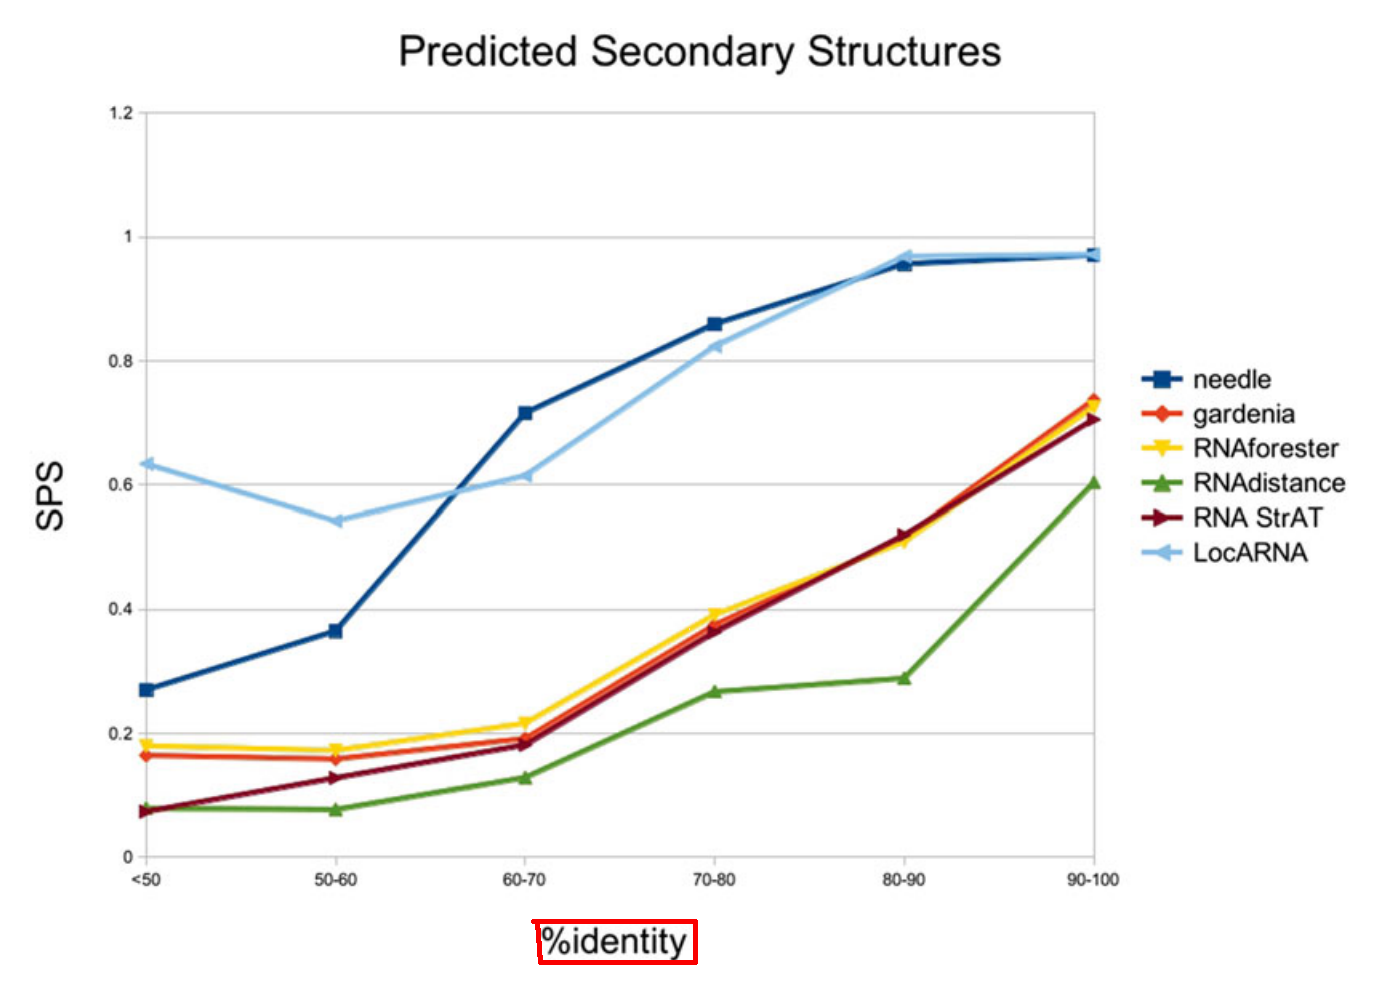
\includegraphics[width=\textwidth]{predicted_identity}
\end{frame}


\begin{frame}[c]{Sequence Identity - Example}
    A: \only<4-5>{AAGGC}\only<1-1>{AAGGC}\only<2-3>{{\color{ForestGreen} AAGGC}}TT \\
    B: \only<1-1>{AAGGC}\only<2-5>{{\color{ForestGreen} AAGGC}} \\
    C: \only<1-3>{AAGGC}\only<4-5>{{\color{ForestGreen} AAGGC}}AT \newline
    \newline
    Identity: \only<3,5>{100\%} \\
    Identical nucleotides / shorter sequence length
\end{frame}


\begin{frame}[c]{Sequence Identity - Example}
    A: {\color{ForestGreen}AAGGC}{\color{red}T}{\color{ForestGreen}T} \\
    B: AAGGC \\
    C: {\color{ForestGreen}AAGGC}{\color{red}A}{\color{ForestGreen}T} \newline
    \newline
    Identity: \only<2>{85\% = 6 / 7} \\
    Identical nucleotides / shorter sequence length
\end{frame}


\begin{frame}[c]{needle}
    \center
    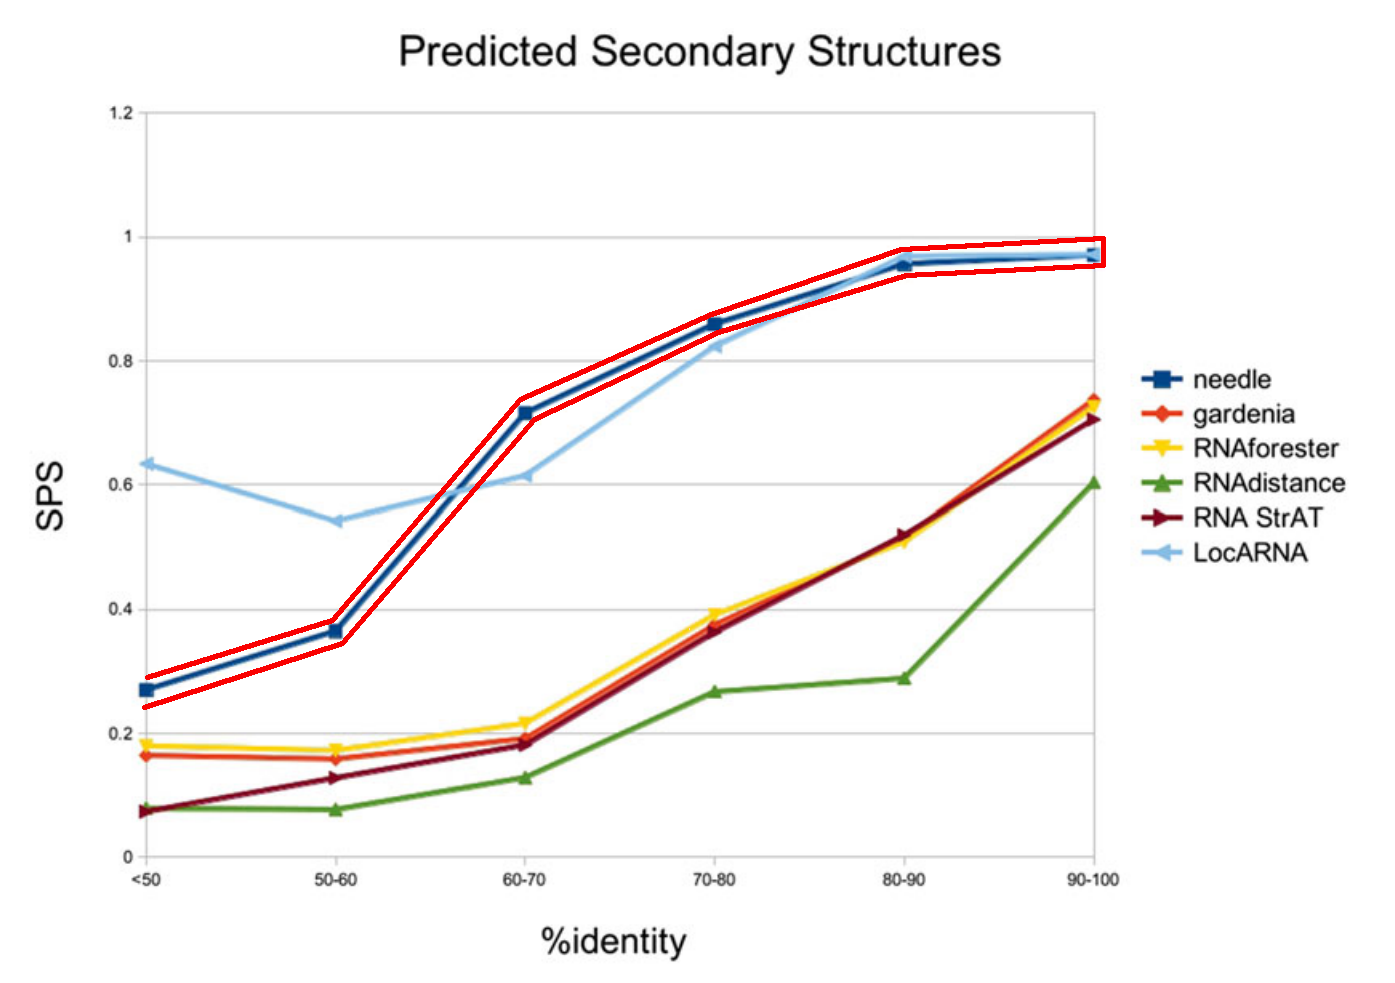
\includegraphics[width=\textwidth]{predicted_needle}
\end{frame}

\begin{frame}[c]{Needleman-Wunsch-Algorithm}
    \center
    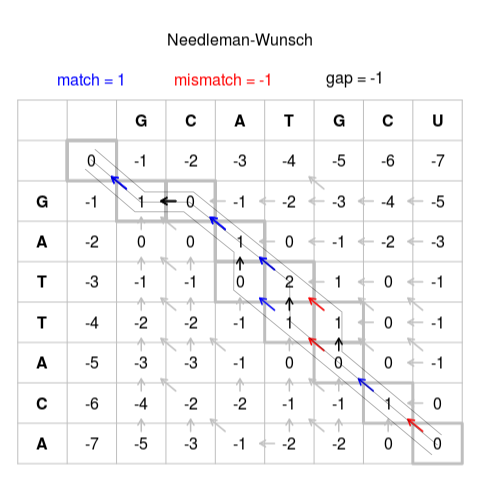
\includegraphics[width=0.75\textwidth]{Needleman-Wunsch_pairwise_sequence_alignment}
\end{frame}











 % PROGRESS

%%%%%%%%%%%%%%%%%%%%%%%%%%%%%%%%%%%%%%%%%%%%%%%%%%CACHED THOUGHTS%%%%%%%%%%%%%%%%%%%%%%%%%%%%%%%%%%%%%%%%%%%%%%%%%%


\section{Cached Thoughts}

\begin{frame}[c]{Cached Thoughts}
    \Large
    Was sind das?
    % Man meint etwas verstanden zu haben, merkt allerdings
    % eines Tages dass man vollkommen falsch lag und dass
    % eigentlich sehr gut selber darauf hätte kommen können
\end{frame}


\begin{frame}[standout]
    Wer hält Strategie für wichtig?
\end{frame}

\begin{frame}[standout]
    \LARGE
    Wer hat sich bereits ernsthaft damit auseinandergesetzt?
\end{frame}



 % DONE

%%%%%%%%%%%%%%%%%%%%%%%%%%%%%%%%%%%%%%%%%%%%%%%%%%NICHT-STRATEGIE%%%%%%%%%%%%%%%%%%%%%%%%%%%%%%%%%%%%%%%%%%%%%%%%%%
% not as important.

%%%%%%%%%%%%%%%%%%%%%%%%%%%%%%%%%%%%%%%%%%%%%%%%%%%ECHTE STRATEGIE%%%%%%%%%%%%%%%%%%%%%%%%%%%%%%%%%%%%%%%%%%%%%%%%%
\section{Echte Strategie}

\begin{frame}[c]{Strategie}
    \Large
    Ein Ziel ist das Was. \\
    Gründe sind das Warum. \\
    \pause
    Strategie ist das Wie.
\end{frame}


\subsection{Kernel}


\begin{frame}[c]{Kernel - was ist das}
    \Large
    Jede gute Strategie hat eine gemeinsame zugrundeliegende Struktur
\end{frame}


\begin{frame}[c]{Kernel - besteht aus}
    \Large
    \begin{itemize}
        \item Diagnose
            \pause
        \item Eine Leitende Idee
            \pause
        \item Menge Zusammenhängender Aktionen
    \end{itemize}
    % Bsp:
    % - Arzt
    % - Autofahren
\end{frame}


\begin{frame}[c]{Kernel - unerwähnt}
    \Large
    \begin{itemize}
        \item Visionen
        \item Hierarchien
            \pause
        \item Ziele
        \item Zeitspannen
            \pause
        \item Reichweite
        \item weiteres ...
%        \item Ideen zur Veränderung
    \end{itemize}
    % Explizit unerwähnt, da nicht teil der Grundstruktur
\end{frame}


\subsection{Diagnose}


\begin{frame}[c]{Kernel - Diagnose}
    \Huge
    Die Große Frage: \\
    \pause
    Was passiert hier eigentlich?
\end{frame}


\begin{frame}[c]{Wirklich die richtige Situation sehen}
    \Huge
    Erinnert ihr euch an Cached Thoughts?
\end{frame}


\begin{frame}[c]{Das Bayes'sche Theorem}
    \Large
    \[
        P(A|X) = \frac{P(X|A) * P(A)}{P(X|A) * P(A) + P(X|\neg A) * P(\neg A)}
    \]
\end{frame}


\begin{frame}[c]{Bayes'sche Theorem: xkcd}
    \begin{multicols}{2}
    \begin{itemize}
        \item[]<1> 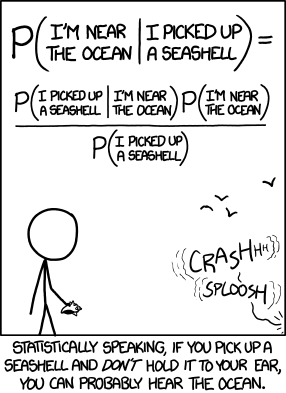
\includegraphics[height=7cm]{xkcd_seashell.png}
        \item[]<2> 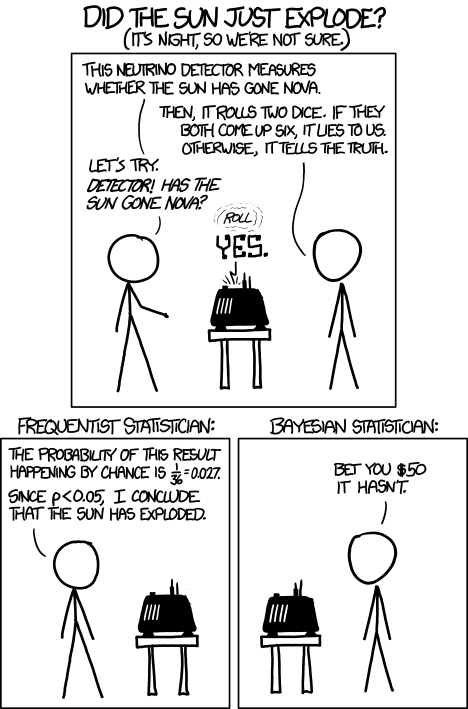
\includegraphics[height=7cm]{xkcd_frequentists_vs_bayesians.png}
    \end{itemize}
    \end{multicols}
\end{frame}


\begin{frame}[standout]
    Ist es möglich dass es anders ist als es scheint?
    % Notes:
    % Bsp:
    % Kein Event bevorzugen,
    % andere, gleichwahrscheinliche beachten
    % Aha-Moment sonst nicht möglich
    % Genauso: Erkennen der eigentlichen Situation
\end{frame}


%
% \begin{frame}[c]{Diagnose - Beispiel}
%     \Large
%     Situation: IBM, 1993, es ging Bergab. \\
%     Diagnose: Zu groß. \\ \pause
%     Neue Diagnose: Zu wenig vernetzt.
%     % TODO: different example
% \end{frame}
%

\begin{frame}[c]{Diagnose - Beispiel}
    \Large
    Situation: Mann liegt am Straßenrand
    % Correspondence Bias
    % TODO: look it up again
\end{frame}

\subsection{Leitidee}


\begin{frame}[c]{Leitidee - Was ist das}
    \Large
    Die grobe richtung, {\em WIE} man weiter vorgeht.
\end{frame}


\begin{frame}[c]{Leitidee - Beispiel}
    \Large
    Situation: Kleiner Eckladen
    % A lot of questions:
    % * More chepaer stuff or more organic stuff?
    % * stock for asian students?
    % * open longer?
    % * more friendly staff?
    % * open longer?
    % * second check-out booth?
    % * parking in the alley?
    % * Paint ceiling white or green?
    % * advertising? what?
    % * what else?
\end{frame}


\subsection{Zusammenhängende Aktionen}


\begin{frame}[c]{Menge Zusammenhängender Aktionen}
    \Huge
    Klingt einfach. Ist es nicht.
    % eigentliche Strategie
\end{frame}


\begin{frame}[c]{Menge Zusammenhängender Aktionen}
    \Huge
    Eigentlicher Teil der Strategie
\end{frame}


\begin{frame}[c]{Menge Zusammenhängender Aktionen}
    \Huge
    Koordinierte Aktionen
\end{frame}


\subsection{Fazit}


\begin{frame}[c]{Kernel}
    \Large
    \begin{itemize}
            \pause
        \item Diagnose
            \pause
        \item Eine Leitende Idee
            \pause
        \item Menge Zusammenhängender Aktionen
    \end{itemize}
    % Bsp:
    % - Arzt
    % - Autofahren
\end{frame}


\begin{frame}[c]{Kernel - Fazit}
    \Large
    Sehr wichtige Grundbausteine, \\
    Sehr vieles wird schiefgehen sollten diese nicht vorhanden sein.
\end{frame}






   % DONE

\section{Vorteilsquellen}

\begin{frame}[c]{Die Zukunft Vorhersagen}
    \Huge
    \pause
    Können wir.
\end{frame}


\begin{frame}[c]{Vorteilsarten}
    \Large
    \begin{itemize}
        \item Hebelwirkung
        \item Erreichbare Ziele
            \pause
        \item Starke Position
        \item Hierarchische Ziele
            \pause
        \item Design
        \item Fokus
%        \item (Wachstum)
%        \item (Entropie)
%        \item (Vorteil)
    \end{itemize}
\end{frame}



\begin{frame}[c]{Vorteil: Hebelwirkung}
    \Large
    Kann sein: Situation zum eigenen Vorteil verwenden. \\
    Wichtig: Kritische Punkte (Diagnose!!).
\end{frame}


\begin{frame}[c]{Vorteil: Erreichbare Ziele}
    \Large
    Situation: Mondlandung \\
\end{frame}

\begin{frame}[c]{Vorteil: Starke Position}
    \Large
    Situation: Schachspiel
\end{frame}


\begin{frame}[c]{Vorteil: Hierarchische Ziele}
    \Large
    Situation: Helikopter meistern
\end{frame}


% \begin{frame}[c]{Cached Thoughts: Hierarchisch}
%     \large
%     Leicht unterschiedliche Situation verändert alles
% \end{frame}


\section{Verkettete Systeme}


\begin{frame}[c]{Verkettete Systeme}
    \Large
    Situation: Space Shuttle Challenger \\
    \pause
    Situation: Fähigkeiten
\end{frame}


\begin{frame}[c]{Verkettete Systeme: Verbesserungen}
    \large
    Inkrementelle Verbesserungen helfen (meist) wenig.
\end{frame}


\begin{frame}[c]{Verkettetes System: Beispiel}
    \Large
    Situation: IKEA
    % Einzlne Links:
    %   large inventory
    %   own stores
    %   own designs
    %   catalogue
    %   logistics
    %   ...
\end{frame}




  % IN PROGRESS
\section{Design}


\begin{frame}[c]{Design}
    \large
    Meister-Strategen sind keine Entscheidungstreffer. \\
    \pause \LARGE
    Sie sind Designer.
\end{frame}


\begin{frame}[c]{Design - Beispiel}
    \Large
    Situation: Schlacht von Cannae
\end{frame}


\begin{frame}[c]{Schlacht von Cannae}
    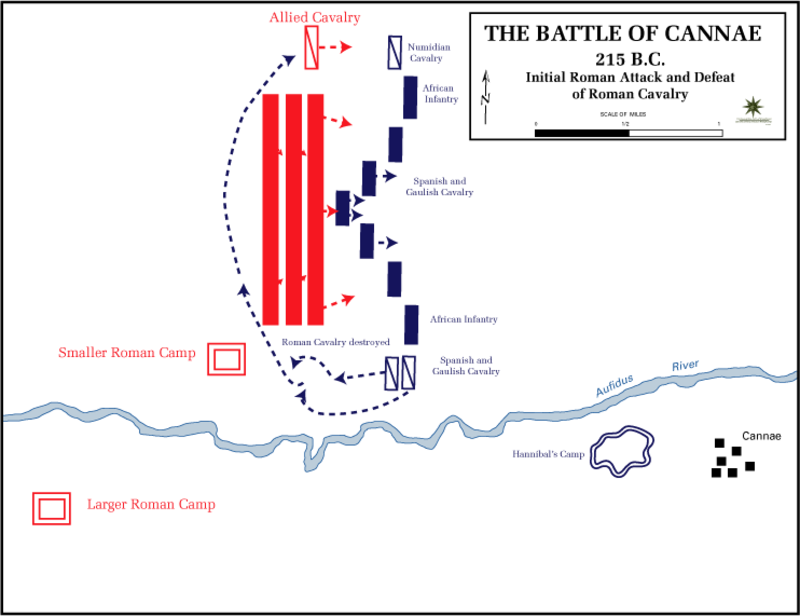
\includegraphics[height=4cm]{strategy/Initial_Roman_attack.png}
    \pause
    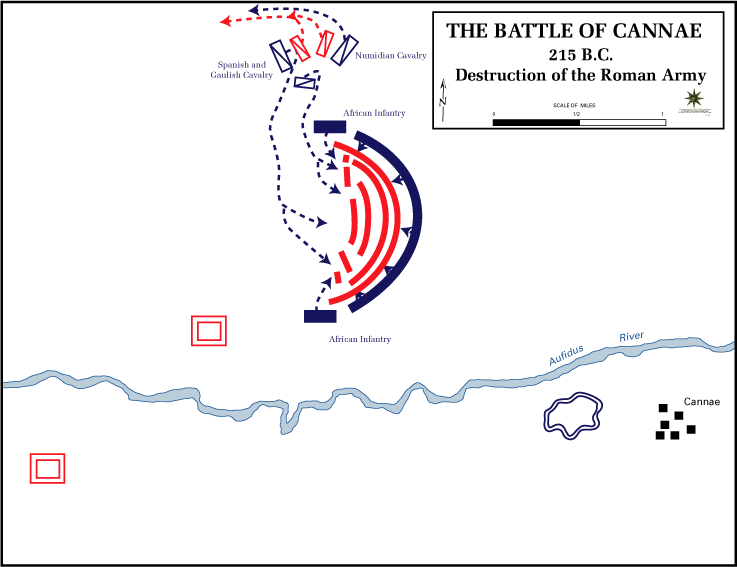
\includegraphics[height=4cm]{strategy/Battle_cannae_destruction.png}
\end{frame}

\begin{frame}[c]{Design - Eigenschaften}
    \large
    \begin{itemize}
        \item Vorsatz
            \pause
        \item Erwartungen
            \pause
        \item Design Koordinierter Aktionen
            \pause
        \item Die Einzelteile als Ganzes
    \end{itemize}
\end{frame}


\begin{frame}[c]{Design - Beispiel}
    \Large
    Situation: Satelliten Designen \\
    \pause
    Performanz ist die Vereinigung von \\
    Ressourcen und gutem Design.
\end{frame}


\begin{frame}[c]{Design - Beispiel}
    \Large
    Situation: Formel 1 vs Normales Auto
\end{frame}


% \begin{frame}[c]{Design - Realität}
%     \large
%     What is true is already so. \\
%     Owning up to it doesn't make it worse. \\ \pause
%     Not being open about it doesn't make it go away. \\ \pause
%     And because it's true, \\
%     it is what is there to be interacted with. \\ \pause
%     Anything untrue isn't there to be lived. \\ \pause
%     People can stand what is true, \\
%     for they are already enduring it.
% \end{frame}
%
% \begin{frame}[c]{Design - Realität}
%     \large
%     Was wahr ist ist es bereits. \\
%     Das zu akzeptieren macht es nicht schlimmer. \\
%     Es nicht zuzugeben lässt es nicht verschwinden. \\
%     Und weil es Wahr ist, \\
%     ist es das was da ist um damit zu Interagieren. \\
%     Alles unwahre ist nicht in der lage gelebt zu werden. \\
%     Alle Menschen können die Wahrheit aushalten, \\
%     ertragen müssen sie sie bereits.
% \end{frame}
%

\begin{frame}[c]{Design - Finden}
    \Large
    Strategie lernen ...
\end{frame}
    % IN PROGRESS
\section{Fokus}

\begin{frame}[c]{Fokus}
    \Huge
    Fokus ist wichtig!
\end{frame}


\begin{frame}[c]{Fokus}
    \Huge
    Important vs Urgent
\end{frame}


\begin{frame}[standout]
    \Huge
    Nein sagen.
\end{frame}


\begin{frame}[c]{Fokus - Beispiel}
    \Large
    Situation: Crown Cork \& Seal
\end{frame}




   % IN PROGRESS
% \section{Die Gleichheit der Menschen}


\begin{frame}[c]{Was ist Gleichheit zwischen Menschen?}
    \Large
    Mehr als nur Gleichheit zwischen Äpfeln. \\ \pause
    Weil Menschen so viel mehr Eigenschaften haben.
\end{frame}


\begin{frame}[c]{Sind Menschen wirklich Gleich?}
    \Large

    Nein sind wir nicht.

    \begin{itemize}
            \pause
        \item Genderfeindlich
            \pause
        \item Ignorant
            \pause
        \item Arrogant
            \pause
        \item Inkonsistent
    \end{itemize}

\end{frame}


\begin{frame}[c]{Zitat von Fukuzawa Yukichi}
    \Large
    It is said that heaven does not create one man above or below another man.
    Any existing distinction between the wise and the stupid, between the rich
    and the poor, comes down to a matter of education.
\end{frame}


\begin{frame}[c]{Gleichheit zwischen Menschen}
    \Large
    Versteht mich nicht falsch, das heißt immernoch dass alle Menschen (z.B. vor
    Gericht) gleich Behandelt werden sollen, also den Umständen entsprechend.
\end{frame}


\begin{frame}[c]{Utilitarismus}
    \Large
    Idee: Es soll allen Menschen möglichst gut gehen.
\end{frame}








 % IN PROGRESS % can not be shown .
\section{Vorteile}

\subsection{Eigenschaften von Vorteilen}

\begin{frame}[c]{Vorteile - Den Gorilla Bekämpfen}
    \Large
    Situation: Textil-Startup
\end{frame}

\begin{frame}[c]{Interessante Vorteile}
    \Large
    Situation: Silbermaschine
\end{frame}


\begin{frame}[c]{Vorteile ausbauen}
    \Large
    \begin{itemize}
        \item Vorteile Vertiefen
        \item Den effekt gewisser Vorteile erweitern
        \item Bestehende Vorteile besser integrieren
            \pause
        \item (Isoliermechanismen für bestehende Vorteile ausbauen)
    \end{itemize}
\end{frame}

\subsection{Vorteile verstehen}

\begin{frame}[c]{Vorteile Vertiefen}
    \Large
    Verbesserung ist kein 'natürlicher' Prozess. \\
    Irrglaube: passiert durch Druck oder Anreize von alleine. \\ \pause
    Beispiel: Mauerbau
\end{frame}


\begin{frame}[c]{Maerbau: Veränderungen}
    \Large
    \begin{itemize}
        \item Vorratspaletten mit Bausteinen auf Brusthöhe
        \item Bewegbare Gerüste
        \item Konsistenz des Mörtels
    \end{itemize}
\end{frame}


\begin{frame}[c]{Vorteile neu entdecken}
    \Large
    Reengineering: Das Rad neu Erfinden \\ \pause
    Ihr erinnert euch an Cached Thoughts?
\end{frame}



   % IN PROGRESS
\section{Dynamik}


\begin{frame}[c]{Klassische Militärstrategie}
    \Large
    Hohen Grund verteidigen. \\ \pause
    Wie findet man also noch nicht besetzten Hohen Grund?
\end{frame}


\begin{frame}[c]{Dynamik}
    \Large
    Man erschafft sich selber welchen!
\end{frame}


\begin{frame}[c]{Dynamik - Beispiel}
    \Large
    Situation: Cisco in 1996. \\
    Eigentliches Schlachtfeld von IBM und AT\&T.
\end{frame}


\begin{frame}[c]{Dynamik}
    \Large
    Auch in anderen Feldern: \\
    Vorteile durch Software
\end{frame}



\begin{frame}[c]{Der Erfolg von Intel}
    \Large
    Situation: Intels 4-bit 4004 Mikroprozessor mit 2300 Transistoren (1971) \\ \pause
    Situation: Intels 8-bit 8008 Mikroprozessor mit 3500 Transistoren (1972)
\end{frame}


\begin{frame}[c]{Dynamik - Design - Kosten}
    \Large
    Situation: (Rolls-Royce) Treibstoffüberwachung für Turbinen
\end{frame}


\begin{frame}[c]{Software vs Hardware}
    \Large
    Hardware ist immer der Limitierende (schnellere) Faktor.
\end{frame}


\begin{frame}[c]{Dynamik - Beispiel}
    \Large
    Situation: Dekonstruktion der Computerindustrie.
\end{frame}


% TODO: update
\begin{frame}[c]{Dynamik - Cisco detailliert/ursprünge}
    \Large

    Veränderungen die Cisco ausgenutzt hat:
    \begin{itemize}
        \item Mikroprozessoren und Kritikalität der Software-Skills
            \pause
        \item Firmen wollten sich mehr und mehr verknüpfen (verschiedene Protokolle)
            \pause
        \item Die ursprünge des Internets (bzw. IP)
            \pause
        \item Das Internet wurde für alle Zugänglich
    \end{itemize}

    % critical rise of need for software-related skill
    % increase in corporate data networking
    % unifying IP -> shift
    % exploding internet

    % Microprocessor and Key implication: Software centrality
    % Corporate Networking: Different Protocols
    % Rise of IP - SNA, DECnet, AppleTalk, Ethernet, NetBIOS
\end{frame}


\begin{frame}[c]{Dynamik - Indikatoren für Veränderungen}
    \Large

    \begin{itemize}
        \item Steigende Konstante Kosten
            \pause
        \item (Deregulation)
            \pause
        \item Vorurteilsbehaftete Vorhersagen
            \pause
        \item Verspätete Antworten
            \pause
        \item 'Scheinbar' Stabile Zustände
    \end{itemize}
\end{frame}



 % IN PROGRESS
\section{Trägheit und Entropie}


\begin{frame}[c]{Trägheit}
    \Large
    Erstes Newtonsches Gesetz!
\end{frame}


\begin{frame}[c]{Entropie}
    \Large
    Zweites Thermodynamische Gesetz: \\
    Die Entropie eines geschlossenen Systems strebt immer zum Maximum!
\end{frame}


\begin{frame}[c]{Wichtige Implikationen für Strategie}
    \Large
    Gibt es auch bei Firmen! \\ \pause
    Situation: Mobile OS und Microsoft

\end{frame}


\begin{frame}[c]{Trägheit: Routine}
    \Large
    Situation: Luftlinien-Deregulation in Amerika, 1978
    % 0.22$ vs 0.09$ per ASM
    % weiterverwendung der selben software zum Bestimmen von Preisen.
\end{frame}


\begin{frame}[c]{Trägheit: Kultur}
    \Large
    Situation: Bell Labs
    % inventor of the Transistor, the C Programming Language, Unix, it brought several Nobel-Prizes in, ...
\end{frame}


\begin{frame}[c]{Entropie: Beispiel}
    \Large
    Situation: General Motors
\end{frame}


 % TODO
\section{Nvidia}

\begin{frame}[c]{Warum Nvidia als Beispiel?}
    \Large
    Grund: Nvidias Aufstieg ist hauptsächlich guter Strategie zu verdanken
\end{frame}



\begin{frame}[c]{3D-Graphik Situation}
    \Large
    \begin{itemize}
        \item Graphics Pipeline \& GL
            \pause
        \item Reality Engine
            \pause
        \item Doom \& Quake
            \pause
        \item 3dfx
            \pause
        \item NV1: Multimedia-Plattform
            \pause
    \end{itemize}
\end{frame}


\begin{frame}[c]{Nvidias Aufstieg}
    \Large
    \begin{itemize}
        \item Moores Law
            \pause
        \item DirectX
            \pause
        \item Design-Tools
            \pause
        \item Treiber
            \pause
        \item Nur-Design
    \end{itemize}
\end{frame}



 % TODO



% * Thinking about thinking
% * Tools
% * Motivated stopping
% * Relationship of Strategy and Science
% * Relationship of Strategy and Rationality
% * Terminologies of Rationality
% * a few more things Rationality says (Occam's Razor?)




\section{SpaceX}

\begin{frame}[c]{SpaceX - Gründung}
    \Large
    Gegründet: 6. Mai 2002 (vor 15 Jahren) \\ \pause
    Warum überhaupt? \pause
    Diagnose.
\end{frame}

\begin{frame}[c]{SpaceX - Ziele}
    \Large
    Bringe 1'000'000 Menschen auf den Mars.
\end{frame}


\begin{frame}[c]{SpaceX - Aktionen}
    \Large
    \begin{itemize}
        \item Rakete gebaut und Orbit erreicht.
            \pause
        \item Transporter gebaut und getestet.
            \pause
        \item ISS beliefert (Kunden bekommen).
            \pause
        \item Satelliten Transportieren.
            \pause
        \item Erste Stufe landen.
            \pause
        \item Erste Stufe zweimal fliegen lassen.
            \pause
        \item Weitere Teile Wiederverwenden.
            \pause
        \item Transporter nochmal fliegen lassen.
    \end{itemize}
\end{frame}



 % TODO

%%%%%%%%%%%%%%%%%%%%%%%%%%%%%%%%%%%%%%%%%%%%%%%%%%BEISPIELE FÜR GUTE STRATEGIE%%%%%%%%%%%%%%%%%%%%%%%%%%%%%%%%%%%%%
% % Mabye this is unnecessary, or rather, should already be included as examples all over

 % IN PROGRESS - Required even ?

%%%%%%%%%%%%%%%%%%%%%%%%%%%%%%%%%%%%%%%%%%%%%%%%%%%%%%%%%%%%%%%%%%%%%%%%%%%%%%%%%%%%%%%%%%%%%%%%%%%%%%%%%%%%%%%%%%%
%%%%%%%%%%%%%%%%%%%%%%%%%%%%%%%%%%%%%%%%%%%%%%%%%%%%%%%%%%%%%%%%%%%%%%%%%%%%%%%%%%%%%%%%%%%%%%%%%%%%%%%%%%%%%%%%%%%

%%%%%%%%%%%%%%%%%%%%%%%%%%%%%%%%%%%%%%%%%%%%%%%%%%CITES%%%%%%%%%%%%%%%%%%%%%%%%%%%%%%%%%%%%%%%%%%%%%%%%%%%%%%%%%%%%
\ifEnglish
%%%%%%%%%%%%%%%%%%%%%%%%%%%%%%%%%%%%%%%%%%%%%%%%%%%%%%%%%%%%

\section{Sources}

\begin{frame}[c]
    
\end{frame}



%%%%%%%%%%%%%%%%%%%%%%%%%%%%%%%%%%%%%%%%%%%%%%%%%%%%%%%%%%%%
\else
%%%%%%%%%%%%%%%%%%%%%%%%%%%%%%%%%%%%%%%%%%%%%%%%%%%%%%%%%%%%


%%%%%%%%%%%%%%%%%%%%%%%%%%CITES%%%%%%%%%%%%%%%%%%%%%%%%%%%%%
\section{Quellen}

%%%%%%%%%%%%%%%%%%%%%%%%%%CITES%%%%%%%%%%%%%%%%%%%%%%%%%%%%%
\begin{frame}[c,fragile,allowframebreaks]{Quellen}
    Die Folien sind zu finden unter: \newline
    \url{https://github.com/fkarg/things-to-talk-about/tree/master/lesswrong}
    \newline
    \newline
    Das Forum, mit diesen und sehr viel mehr Themen: \newline

% 
% 
%     Das Buch, aus dem ich den Vortrag gebastelt hab:
% 
    \beamertemplatearticlebibitems
    \begin{thebibliography}{10}
    \bibitem{Less Wrong}
            {\bf Less Wrong}
            \newblock \url{http://lesswrong.com/}

%     \beamertemplatebookbibitems
%     \bibitem{Richard Rumelt}
%         Richard Rumelt
%         \newblock {\em Good Strategy / Bad Strategy}.
%         \newblock The Difference and Why It Matters \\
%                   ISBN: 978-1-78125-154-6
%     \beamertemplatearticlebibitems
%     \bibitem{Lesswrong}
%         Lesswrong
%             \newblock {\em Expecting short Inferential Distances}
%             \newblock \url{http://lesswrong.com/lw/kg/expecting\_short\_inferential\_distances/}
%     \bibitem{Lesswrong}
%         Lesswrong
%             \newblock {\em Cached Thoughts}
%             \newblock \url{http://lesswrong.com/lw/k5/cached\_thoughts/}
%     \bibitem{Zenhabits}
%         Zenhabits
%             \newblock {\em say No so you can say YES}
%             \newblock \url{https://zenhabits.net/say-yes/}
% 
%     \bibitem{Wikiquote}
%         Fukuzawa Yukichi
%             \newblock {\em Wikiquote}
%             \newblock \url{https://en.wikiquote.org/wiki/Fukuzawa\_Yukichi}
% 
%     \bibitem{SpaceX}
%         SpaceX
%             \newblock {\em SpaceX}
%             \newblock \url{http://www.spacex.com/}
% 
%    \bibitem{Wihipedia}
%        Wikipedia
%            \newblock {\em Proton-M}
%            \newblock \url{https://en.wikipedia.org/wiki/Proton-M}
%    \bibitem{Wikipedia}
%        Wikipedia
%            \newblock {\em Ariane 5}
%            \newblock \url{https://en.wikipedia.org/wiki/Ariane\_5}
%    \bibitem{Wikipedia}
%        Wikipedia
%            \newblock {\em Delta IV Heavy}
%            \newblock \url{https://en.wikipedia.org/wiki/Delta\_IV}
   \end{thebibliography}
    % required the allowframebreaks for longer lists

\end{frame}



%%%%%%%%%%%%%%%%%%%%%%%%%%%%%%%%%%%%%%%%%%%%%%%%%%%%%%%%%%%%
\fi
 % IN PROGRESS

% other articles to include:
% belief chains: http://lesswrong.com/lw/l9d/belief_chains/
% reversed stupidity? http://lesswrong.com/lw/lw/reversed_stupidity_is_not_intelligence/
% map and territory?



%%%%%%%%%%%%%%%%%%%%%%%%%%%%%%%%%%%%%%%%%%%%%%%%%%%%%%%%%%%%%%%%%%%%%%%%%%%%%%%%%%%%%%%%%%%%%%%%%%%%%%%%%%%%%%%%%%%


\end{document}
